\subsection{Comparator}

\begin{minted}[
   fontsize=\footnotesize,
   linenos,
   breaklines,
]{verilog}
module comparator #(
   parameter bcd_digit_0 = 4'd2,
   parameter bcd_digit_1 = 4'd8,
   parameter bcd_digit_2 = 4'd0,
   parameter bcd_digit_3 = 4'd1
)(
   input [3:0] bcd_0_i,
   input [3:0] bcd_1_i,
   input [3:0] bcd_2_i,
   input [3:0] bcd_3_i,
   output equal_o
);

assign equal_o = &{
   bcd_digit_0 == bcd_0_i,
   bcd_digit_1 == bcd_1_i,
   bcd_digit_2 == bcd_2_i,
   bcd_digit_3 == bcd_3_i
};

endmodule
\end{minted}

\begin{minted}[
   fontsize=\footnotesize,
   linenos,
   breaklines,
]{verilog}
module comparator_tb;

reg [3:0] bcd_0_i;
reg [3:0] bcd_1_i;
reg [3:0] bcd_2_i;
reg [3:0] bcd_3_i;

wire equal_o;

comparator DUT (
   .bcd_0_i(bcd_0_i),
   .bcd_1_i(bcd_1_i),
   .bcd_2_i(bcd_2_i),
   .bcd_3_i(bcd_3_i),
   .equal_o(equal_o)
);

initial begin
   bcd_0_i = 4'd0;
   bcd_1_i = 4'd0;
   bcd_2_i = 4'd0;
   bcd_3_i = 4'd0;
end

initial begin
   #100;

   bcd_0_i = 4'd2;
   bcd_1_i = 4'd8;
   bcd_2_i = 4'd0;
   bcd_3_i = 4'd1;
   #100;

   bcd_0_i = 4'd4;
   bcd_1_i = 4'd4;
   bcd_2_i = 4'd4;
   bcd_3_i = 4'd4;
   #100;

// Finish the Simulation
   #100;
   $finish;
end

endmodule
\end{minted}

\begin{figure}[htbp]
   \centering
   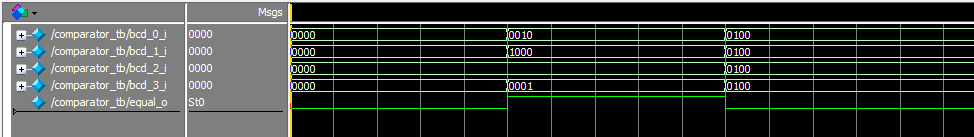
\includegraphics[width=\textwidth]{comparator_sim.png}
   \caption{Testbench simulation of the comparator module.}
   \label{fig:comparator_sim}
\end{figure}
